\documentclass[12pt]{article}
\usepackage{graphicx}
\usepackage{hyperref}
\usepackage[top=2.75in, left=1in, right=1in, bottom=0.25in]{geometry}
\usepackage[utf8]{inputenc}
\usepackage[english]{babel}
\usepackage{fancyhdr}
\usepackage[utf8]{inputenc}
\usepackage{listings}
\usepackage{color}
\usepackage[final]{pdfpages}

\definecolor{codegreen}{rgb}{0,0.6,0}
\definecolor{codegray}{rgb}{0.5,0.5,0.5}
\definecolor{codepurple}{rgb}{0.58,0,0.82}
\definecolor{backcolour}{rgb}{0.95,0.95,0.92} 
\lstdefinestyle{mystyle}{
    backgroundcolor=\color{backcolour},   
    commentstyle=\color{codegreen},
    keywordstyle=\color{magenta},
    numberstyle=\tiny\color{codegray},
    stringstyle=\color{codepurple},
    basicstyle=\footnotesize,
    breakatwhitespace=false,         
    breaklines=true,                 
    captionpos=b,                    
    keepspaces=true,                 
    numbers=left,                    
    numbersep=5pt,                  
    showspaces=false,                
    showstringspaces=false,
    showtabs=false,                  
    tabsize=2
} 
\lstset{style=mystyle}

\setlength{\parindent}{4em}
\setlength{\parskip}{1em}
\pagestyle{fancy}
\fancyhf{}
\rhead{Assignment 2}
\lhead{Huan Huang}
\renewcommand{\headrulewidth}{0.4pt}
\renewcommand{\footrulewidth}{0.4pt}
\rfoot{Page \thepage}


\begin{document}
\begin{titlepage}
	\begin{center}
	\Huge{Web Science cs532-s16}\\
	[0.25in]
	\textsc{\Large Assignment 2 Report}\\
	[4.25in]
	\textsc{\normalsize By: Huan Huang}\\
	\large 02/11/2016\\
	
	
	\end{center}
\end{titlepage}
\newpage

\newgeometry{margin=1in}

\section*{Problem 1}
Write a Python program that extracts 1000 unique links from
Twitter.  You might want to take a look at:

\noindent
http://thomassileo.com/blog/2013/01/25/using-twitter-rest-api-v1-dot-1-with-python/

\noindent
But there are many other similar resources available on the web.  Note
that only Twitter API 1.1 is currently available; version 1 code will
no longer work.

\noindent
Also note that you need to verify that the final target URI (i.e., the
one that responds with a 200) is unique.  You could have many different
shortened URIs for www.cnn.com (t.co, bit.ly, goo.gl, etc.).

\noindent
You might want to use the search feature to find URIs, or you can
pull them from the feed of someone famous (e.g., Tim O'Reilly).

\noindent
Hold on to this collection -- we'll use it later throughout the semester.

\subsection*{Answer}
For this problem, I created 3 programs that handled the problem at each stage. But before I can start writing the programs, I had to register a new application with my twitter account. Once that is approved, I received my keys and tokens, with those keys and tokens I can access twitter's data through its API. So, the purpose of my first program is to use my keys and tokens to access twitter's data and listen for any tweets that contain the subject or phrase I set in my filter. originally, I intended to use Tweepy for this job, then, I came across the another module called Python Twitter Tools which made this part of assignment much simpler. When I setup the API object for tweet streaming, it automatically assign the different parts of the tweet into entities, all I have to do now is call for the entity urls to bring up the links in every tweet. 

\lstinputlisting[language=Python]{Initialurls.py}

I let the program ran for about 30 minutes and collected 3896 links, which I saved in a text file called initialurls.txt(every file I mention will be provided in github).

\begin{figure}[h]
\centering
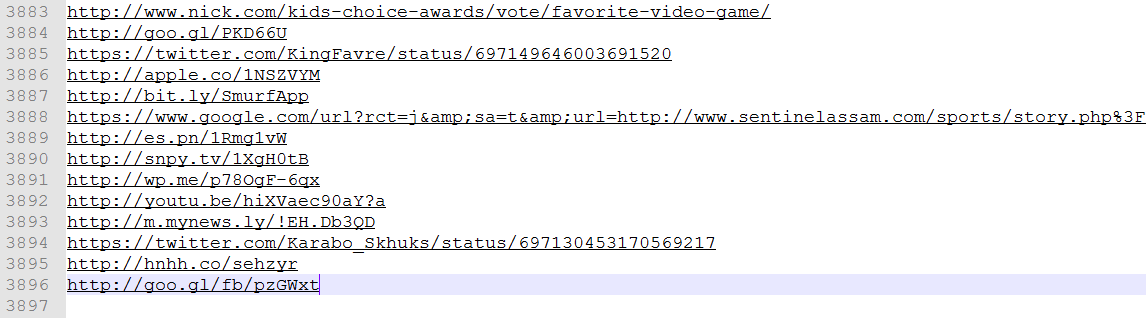
\includegraphics[width=6.5in]{Initialurls.png}
\caption{Sample of part of the initialurls.txt}
\end{figure}
\newpage

Many of these URLs are short links or redirects, to handle that I wrote another program called urlredirect. I actually have two version of this program that does almost the same thing. The other version of this program uses request.get instead of HTTPRedirectHandler. But it operates much slower and sometimes stops at a URL without giving me any error or return control back to me nor was it in an infinite loop. It just stops there and this issue only happens sometimes. I could not figure out why and, therefore, given up on it.

\lstinputlisting[language=Python]{urlredirect.py}

The result is saved in a file called urlsRound2.txt.
\newpage

\begin{figure}[h]
\centering
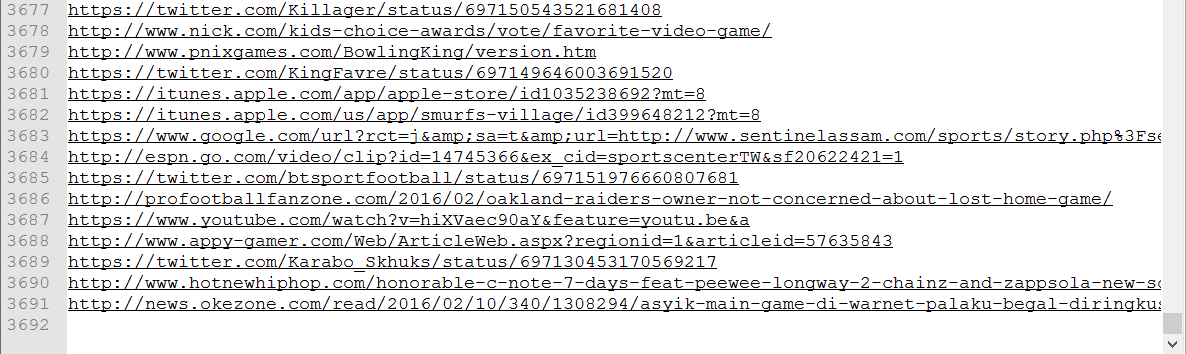
\includegraphics[width=6.5in]{urlround2.png}
\caption{Sample of Part of urlround2.txt}
\end{figure}

The links I have now are all final links that would return a 200 response code, but there are too many duplicates and I only need 1000 unique links. Therefore, I created another program called uniqueurls.py to give me 1000 unique links. It just use \textit{set} function to remove duplicate strings and remove all lines after line 1000.

\lstinputlisting[language=Python]{uniqueurls.py}
\newpage
The final result of 1000 unique URLs are saved in a file called requiredurls.txt. 

\begin{figure}[h]
\centering
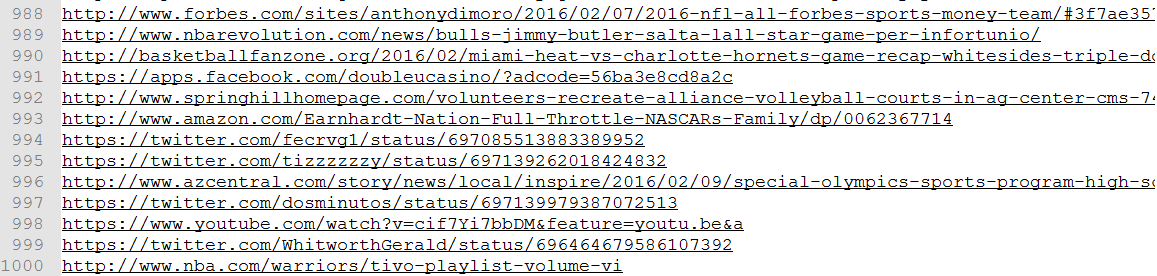
\includegraphics[width=6.5in]{requiredurls.png}
\caption{Sample of part of requiredurls.txt}
\end{figure}

\section*{Problem 2}
Download the TimeMaps for each of the target URIs.  We'll use the ODU 
Memento Aggregator, so for example:

\noindent
URI-R = http://www.cs.odu.edu/

\noindent
URI-T = http://mementoproxy.cs.odu.edu/aggr/timemap/link/1/http://www.cs.odu.edu/

\noindent
Create a histogram* of URIs vs. number of Mementos (as computed from
the TimeMaps).  For example, 100 URIs with 0 Mementos, 300 URIs
with 1 Memento, 400 URIs with 2 Mementos, etc.

\noindent
* = https://en.wikipedia.org/wiki/Histogram
     
\subsection*{Answer}

For this problem, my approach is this, for every link in the 1000 links, attach the url http://mementoproxy.cs.odu.edu/aggr/timemap/link/1/ in front of it. Then, use curl or urllib2.urlopen or whatever to open the newly generated links. (Be careful, if you are using curl, make sure to put the entire url inside ``''.)In the response, whenever the strings rel=``memento", rel=``first memento", rel=``last memento", rel=``memento first", rel=``memento last" appear, it means there is a memento. Therefore, I just have to count them and add them up. Also, the response of some sites may contain the `rel=``timemap"', it means this site have more mementos in another link, make sure to open them up and count the mementos in there as well.

\lstinputlisting[language=Python]{countMomento.py}

The outputs are saved in two files, one contain the count and corresponding links(which is used later in problem 3), and another one only contain the count number(which is used for the graph).

\begin{figure}[h]
\centering
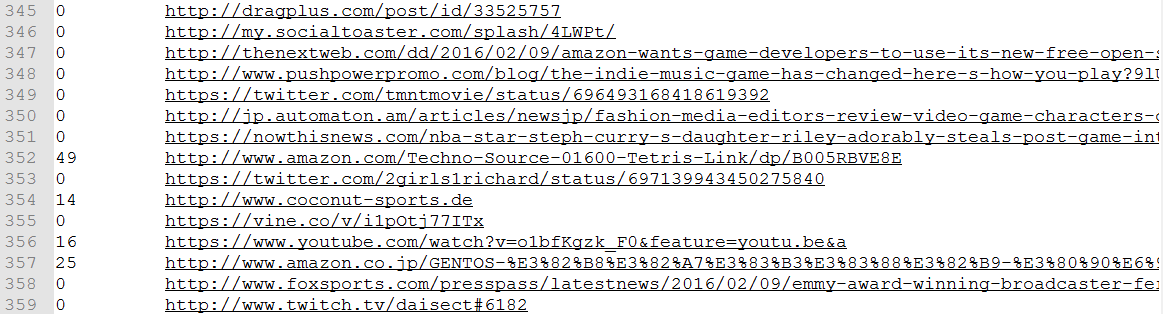
\includegraphics[width=6.5in]{countMomento.png}
\caption{Sample of part of countMemento.txt}
\end{figure}

Below is the R code and graph of the histogram.

\lstinputlisting[language=Python]{histgraph.r}

\newpage

\begin{figure}[h]
\centering
 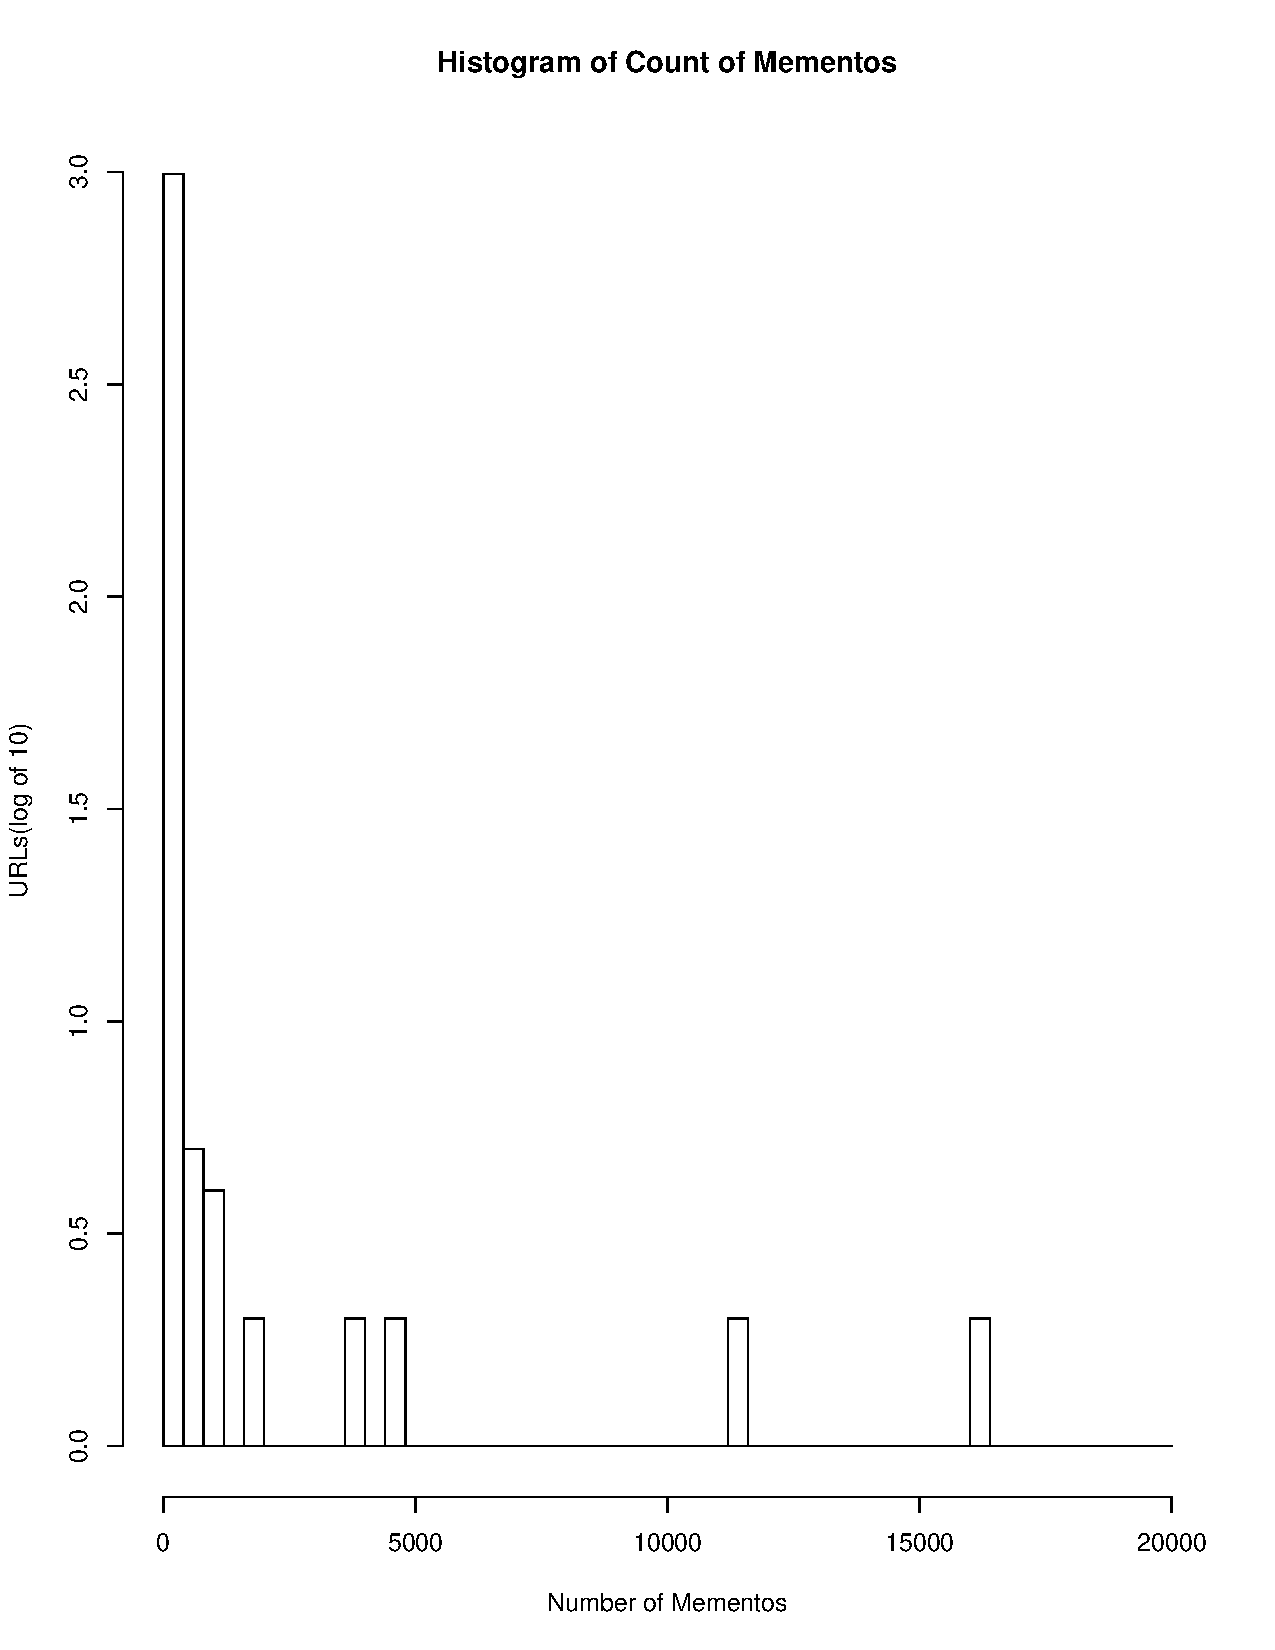
\includegraphics[page=1,
    width=4.5in,
    height=4in]{HistogramofCountofMementos.pdf}
\end{figure}

\section*{Problem 3}
Estimate the age of each of the 1000 URIs using the "Carbon Date" tool:

\noindent
http://ws-dl.blogspot.com/2014/11/2014-11-14-carbon-dating-web-version-20.html

\noindent
Note: you'll should download the library and run it locally; don't
try to use the web service.

\noindent
For URIs that have > 0 Mementos and an estimated creation date,
create a graph with age (in days) on one axis and number of mementos
on the other.  

\noindent
Not all URIs will have Mementos, and not all URIs will have an estimated
creation date.  State how many fall into either categories. 

\subsection*{Answer}
For this problem, we have to create a Bitly account first. While waiting for your verification mail to activate your account, go install PhantomJS, download CasperJS, and download CarbonDate tools. CasperJS is just a compressed folder with some files in it, just put it somewhere you can remember, but make sure you create a short link in /usr/local/bin that points to the casperjs file in the bin fold in the CasperJS folder. Now, activate your Bitly account and generate a token. Open the CarbonDate tool folder and open the config file, put your token in the right place and make sure the ``CasperJSLocation" is set to where you created your short link towards the casperjs file. Now, we can finally start on the program itself. 

To carbon date the 1000 links, I actually went into the local.py file and altered it. Since we are only looking for the estimated creation date, I just have the \textit{cd} function return the variable \textit{lowest}. Once I have the values outside the function, I convert it from string format back to object and use the time of now to subtract it to get the days since the site's creation. The result is saved in carbonDate.txt file.

\lstinputlisting[language=Python]{local.py}

\begin{figure}[h]
\centering
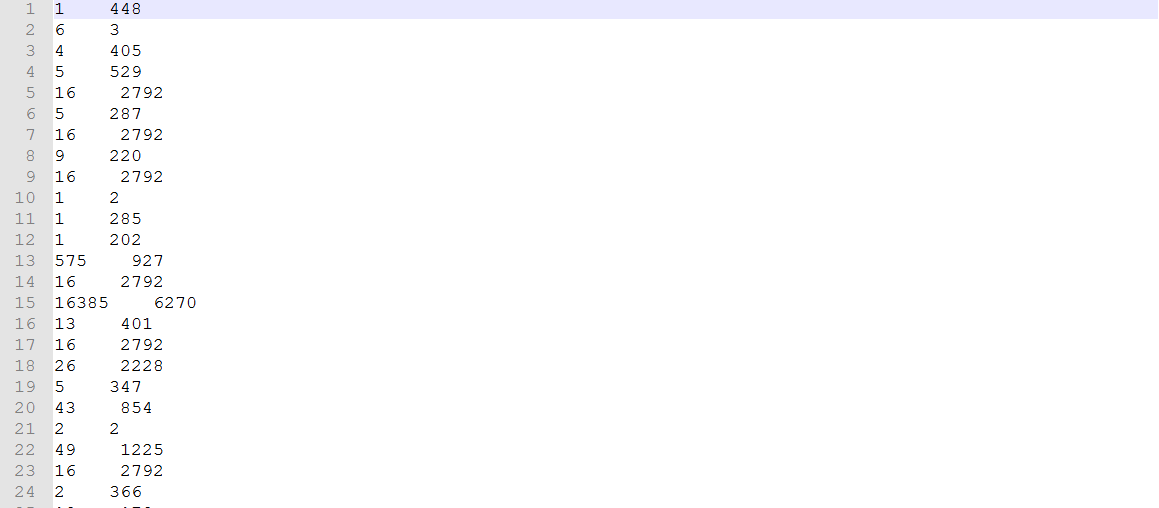
\includegraphics[width=6.5in]{carbonDate.png}
\caption{Sample of part of carbonDate.txt}
\end{figure}
\newpage

Now to finish the problem just use the data in carbonDate.txt to create a graph.

\begin{figure}[h]
\centering
 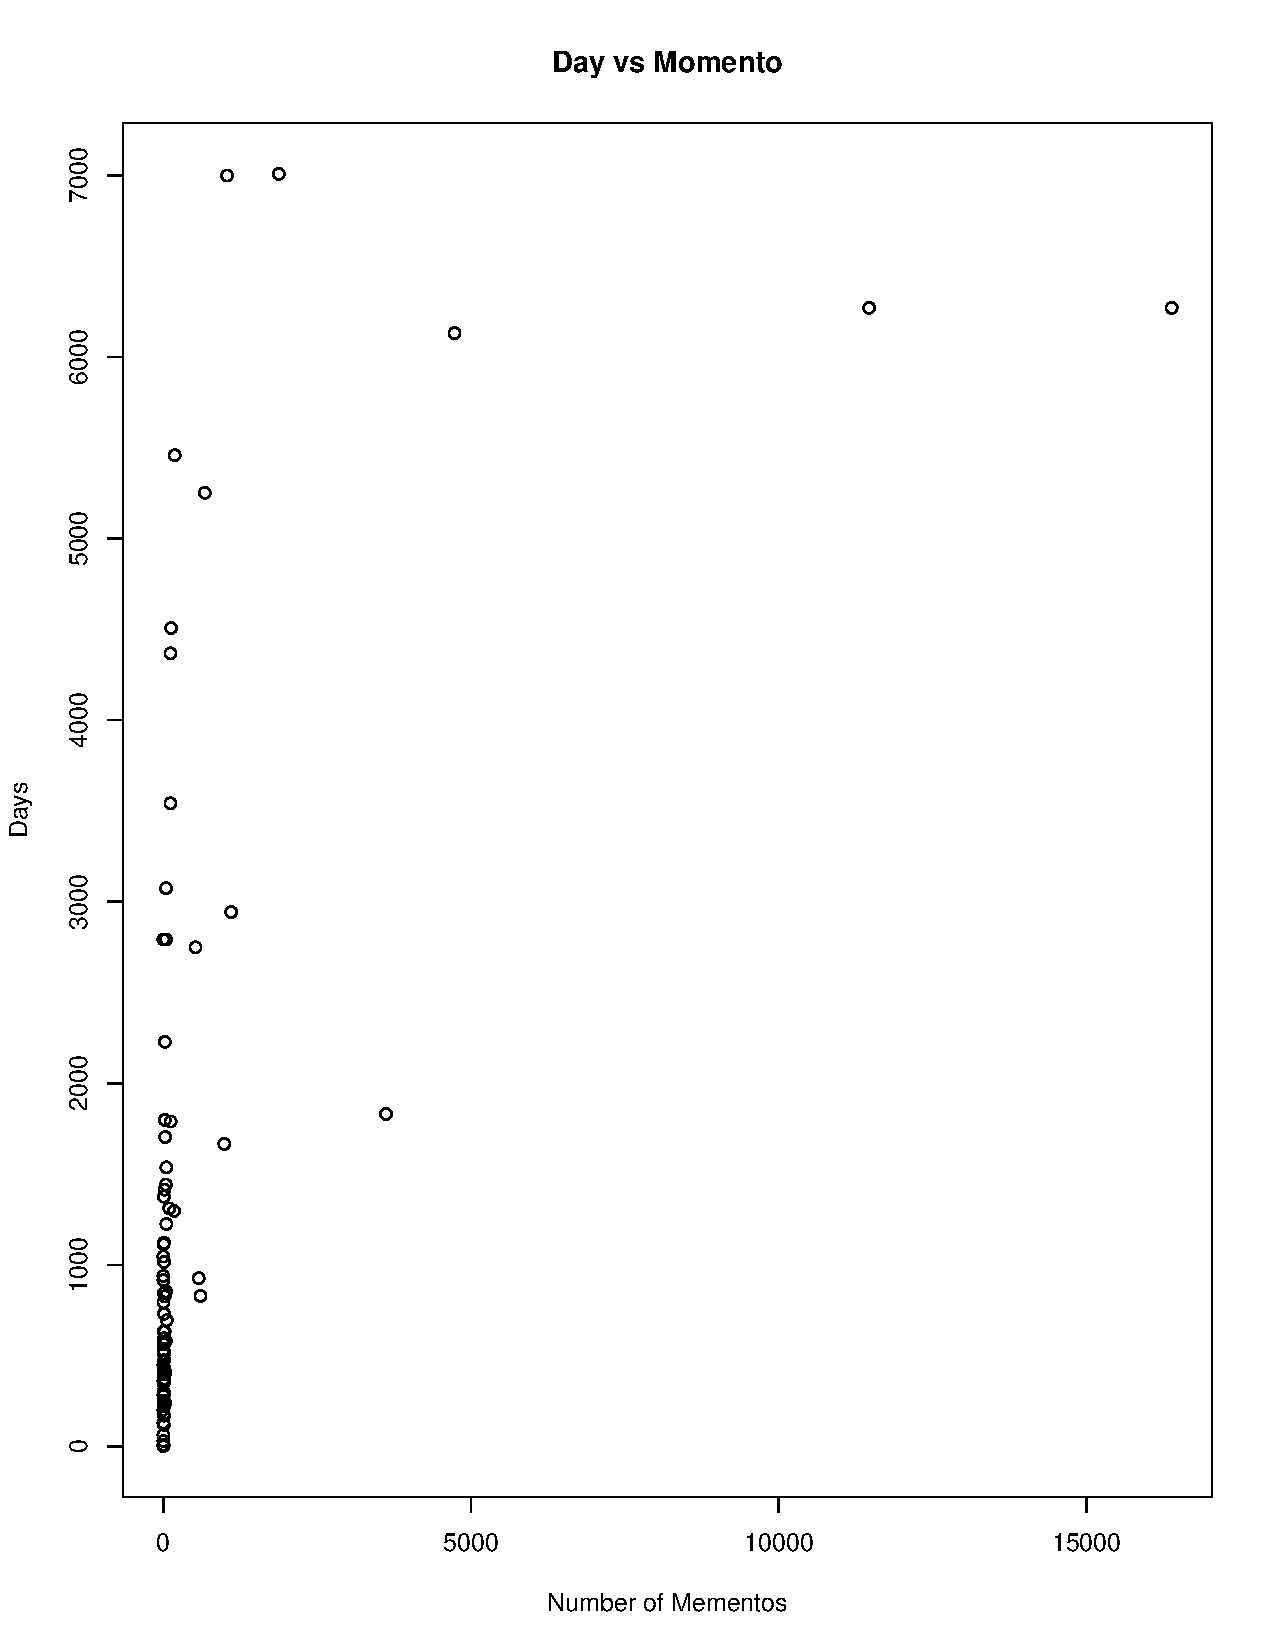
\includegraphics[page=1,
    width=4.5in,
    height=4in]{carbonDate.pdf}
\end{figure}

\end{document}